% !TEX root = ./rapport.tex
% ══════════════════════════════════════════════════════════════════════
%  CHAPITRE 7 — TESTS ET VALIDATION
% ══════════════════════════════════════════════════════════════════════

\chapter{Tests et Validation}

\noindent\textbf{Plan}
\begin{enumerate}
  \item Introduction
  \item Stratégie de test
  \item Tests unitaires, de sécurité et Kafka des microservices
  \item Tests de démarrage du contexte Spring
  \item Tests d'intégration API
  \item Validation des scénarios métier
  \item Bilan de la couverture
  \item Conclusion
\end{enumerate}

% ─────────────────────────────────────────────────────────────
\section{Introduction}
% ─────────────────────────────────────────────────────────────

La validation d'une plateforme GRH repose sur deux exigences contradictoires~:
garantir que chaque règle métier (workflow de validation hiérarchique, calcul
du score d'attrition, progression des projets) est correctement implémentée~;
et maintenir un cycle de développement rapide compatible avec des sprints de deux
semaines. Synapse adopte une stratégie de test à cinq niveaux complémentaires~:
tests unitaires des couches service, tests de sécurité \texttt{@WebMvcTest},
tests d'intégration Kafka \texttt{@EmbeddedKafka}, tests de démarrage du contexte
Spring, et validation des scénarios bout-en-bout sur l'environnement Docker Compose
local. Ce chapitre documente l'ensemble de cette démarche~: les cas de test
implémentés, les métriques de couverture JaCoCo et les résultats obtenus.

% ─────────────────────────────────────────────────────────────
\section{Stratégie de test}
% ─────────────────────────────────────────────────────────────

\subsection{Pyramide de test de Synapse}

La stratégie de test de Synapse suit une pyramide à cinq niveaux~:

\begin{enumerate}[leftmargin=*,nosep]
  \item \textbf{Tests unitaires (base)} — Vingt-six tests JUnit/Mockito couvrent
        les couches service des trois microservices à logique métier complexe~:
        \textit{demandes-service} (workflow de validation hiérarchique, 11 cas),
        \textit{analytics-service} (algorithme de scoring d'attrition, 8 cas) et
        \textit{projets-service} (calcul de progression, cas limites, 7 cas).
        Toutes les dépendances externes (repositories Oracle, producer Kafka,
        API Groq) sont mockées via Mockito~: les tests s'exécutent sans
        infrastructure externe en moins de 2 secondes.
  \item \textbf{Tests de sécurité \texttt{@WebMvcTest}} — Cinq tests automatisés
        (\textit{employe-service}) utilisent \texttt{spring-security-test} et le
        post-processeur \texttt{jwt()} pour vérifier les règles
        \texttt{authorizeHttpRequests()} sans contacter Keycloak~: 401 sans token,
        403 pour rôle insuffisant, 201 pour rôle autorisé.
  \item \textbf{Tests Kafka \texttt{@EmbeddedKafka}} — Deux tests d'intégration
        (\textit{demandes-service}) valident la sérialisation JSON du
        \texttt{NotificationEvent} et le routage par clé \texttt{employeeId}
        sur le topic \texttt{notification-events}, sans broker Docker.
  \item \textbf{Tests de contexte (milieu)} — Sept tests \texttt{@SpringBootTest}
        vérifient que chaque microservice démarre sans erreur dans un contexte Spring
        minimal, sans Oracle ni Keycloak disponibles.
  \item \textbf{Tests d'intégration et bout-en-bout (sommet)} — Douze scénarios
        Postman avec token JWT réel, et quatre scénarios métier complets (congé,
        prêt, attrition, WebSocket) validés sur l'environnement Docker Compose local.
\end{enumerate}

\subsection{Frameworks et outils de test}

\begin{table}[H]
\centering
\caption{Outils de test utilisés dans Synapse}
\label{tab:outils_test}
\begin{tabularx}{\textwidth}{VlVlVLV}
\rowcolor{headerblue!55}
\hline
\textbf{Outil} & \textbf{Version} & \textbf{Rôle} \\
\hline
JUnit 5 & 5.10 (inclus Spring Boot 3.5) & Framework de test unitaire et annotations \texttt{@Test}, \texttt{@DisplayName}, \texttt{@BeforeEach} \\
\hline
Mockito & 5.x & Mock des dépendances (repositories, Kafka, API Groq) via \texttt{@Mock}, \texttt{@InjectMocks} \\
\hline
AssertJ & 3.x & Assertions fluentes (\texttt{assertThat().isEqualTo()}, \texttt{containsExactlyInAnyOrder()}) \\
\hline
Spring Boot Test & 3.5 & Tests de contexte (\texttt{@SpringBootTest}, \texttt{@WebMvcTest}) \\
\hline
spring-security-test & Inclus & \texttt{jwt()} post-processeur pour tester le \texttt{SecurityFilterChain} sans Keycloak \\
\hline
spring-kafka-test & Inclus & \texttt{@EmbeddedKafka} pour tester les producteurs Kafka sans broker réel \\
\hline
JaCoCo & 0.8.11 & Mesure de couverture de code~; rapport HTML/XML généré par \texttt{mvn test} \\
\hline
Postman & 11 & Tests d'API REST manuels avec Bearer token JWT réel \\
\hline
\end{tabularx}
\end{table}

% ─────────────────────────────────────────────────────────────
\section{Tests unitaires des microservices}
% ─────────────────────────────────────────────────────────────

\subsection{Tests unitaires du \textit{demandes-service}}

Le \textit{demandes-service} constitue le cœur logique de Synapse~: il gère cinq
types de demandes et implémente un workflow de validation à plusieurs niveaux
hiérarchiques. La classe \texttt{DemandeServiceTest} couvre onze scénarios unitaires,
chacun isolant la couche service via Mockito~: les cinq repositories Oracle, le
producer Kafka et le service employé sont tous mockés.

\begin{table}[H]
\centering
\caption{Cas de test de \texttt{DemandeServiceTest}}
\label{tab:test_demandes}
\begin{tabularx}{\textwidth}{V>{\centering\arraybackslash}p{0.6cm}VLVLV}
\rowcolor{headerblue!55}
\hline
\textbf{N°} & \textbf{Scénario} & \textbf{Assertion principale} \\
\hline
1 & \texttt{creerDemande(CONGE)} & Sauvegarde dans \texttt{LEAVE\_REQUESTS} avec statut \texttt{EN\_ATTENTE} + autres repos non touchés \\
\hline
2 & \texttt{creerDemande(PRET)} & Sauvegarde dans \texttt{LOAN\_REQUESTS} + aucune interaction avec \texttt{leaveRepo} \\
\hline
3 & Validation congé par Chef & Statut Oracle \texttt{VALIDE\_CHEF}, \texttt{approved\_by = chef\_id}, timestamp non nul \\
\hline
4 & Validation congé par RH & Statut Oracle \texttt{VALIDE\_RH}, \texttt{approved\_by\_rh = rh\_id} \\
\hline
5 & Refus congé par Chef & Statut Oracle \texttt{REFUSE}, \texttt{rejection\_reason} correctement enregistré \\
\hline
6 & Validation formation par Chef & Statut Oracle \texttt{APPROUVE\_CHEF} (différent de \texttt{VALIDE\_CHEF}) \\
\hline
7 & Validation prêt par RH (1\up{er} niveau) & Statut Oracle \texttt{VALIDEE\_DG}~; \texttt{approved\_by\_rh} renseigné (\texttt{needsCommission=false}) \\
\hline
8 & Validation autorisation (flux direct) & Chef → statut \texttt{APPROUVE} directement (pas d'étape intermédiaire) \\
\hline
9 & \texttt{getMesDemandes()} agrégation & Résultat agrège 5 tables, trié du plus récent au plus ancien \\
\hline
10 & Fallback \texttt{resolveEmployeeId} & Recherche par email si \texttt{employee\_id} absent du JWT \\
\hline
11 & Demande introuvable & Lance \texttt{IllegalArgumentException} contenant l'ID, aucun \texttt{save()} émis \\
\hline
\end{tabularx}
\end{table}

\subsection{Setup du contexte de test JWT}

La méthode utilitaire \texttt{buildAuth()} crée un \texttt{JwtAuthenticationToken}
simulant différents profils d'utilisateur (EMPLOYE, CHEF, RH). Le JWT mock porte
le claim \texttt{employee\_id} directement, évitant tout appel Oracle. Cette approche
permet de tester la couche service de manière totalement isolée, sans base de données
ni Keycloak.

\begin{table}[H]
\centering
\caption{JWT de test par profil simulé}
\label{tab:jwt_test}
\begin{tabularx}{\textwidth}{VlVlVlVLV}
\rowcolor{headerblue!55}
\hline
\textbf{Méthode} & \textbf{Subject} & \textbf{Rôle SPRING} & \textbf{Claims supplémentaires} \\
\hline
\texttt{authEmploye()} & \texttt{kc-uuid-emp-010} & \texttt{ROLE\_EMPLOYE} & \texttt{employee\_id = 10, email = nour@gerai.tn} \\
\hline
\texttt{authChef()} & \texttt{kc-uuid-chef-020} & \texttt{ROLE\_CHEF} & \texttt{employee\_id = 20, email = chef@gerai.tn} \\
\hline
\texttt{authRh()} & \texttt{kc-uuid-rh-030} & \texttt{ROLE\_RH} & \texttt{employee\_id = 30, email = rh@gerai.tn} \\
\hline
\end{tabularx}
\end{table}


% ─────────────────────────────────────────────────────────────
\subsection{Tests unitaires de l'\textit{analytics-service} — Algorithme d'attrition}
% ─────────────────────────────────────────────────────────────

Le module de prédiction de l'attrition est le composant à la logique la plus
sensible de Synapse~: un score erroné peut conduire à des décisions RH incorrectes.
La classe \texttt{AttritionScoringServiceTest} couvre huit scénarios unitaires
ciblant les quatre facteurs comportementaux du modèle et leurs interactions.


\begin{table}[H]
\centering
\caption{Cas de test de \texttt{AttritionScoringServiceTest}}
\label{tab:test_attrition}
\begin{tabularx}{\textwidth}{VCVLVLV}
\rowcolor{headerblue!55}
\hline
\textbf{N°} & \textbf{Scénario} & \textbf{Assertion principale} \\
\hline
1 & Employé ancienneté $<$ 6 mois, aucune absence & Score $\geq$ 25, facteur \texttt{ANCIENNETE\_COURTE} présent \\
\hline
2 & Employé avec 30 jours d'absence sur 12 mois & Score augmente de 25~; facteur \texttt{ABSENCES\_ELEVEES} présent \\
\hline
3 & Ratio refus = 2/4 demandes (50\,\%) & Score augmente de 25~; facteur \texttt{DEMANDES\_REFUSEES} présent \\
\hline
4 & Aucune affectation projet active & Score augmente de 25~; facteur \texttt{SOUS\_CHARGE} présent \\
\hline
5 & Cumul des 4 facteurs (profil risque maximal) & Score = 100, niveau \texttt{ELEVE}, liste de 4 facteurs retournée \\
\hline
6 & Employé $>$ 3 ans, 2 congés, 0 refus, projets actifs & Score $\leq$ 5, niveau \texttt{FAIBLE}, liste de facteurs vide \\
\hline
7 & Invalidation du cache après appel \texttt{@CacheEvict} & \texttt{attritionRepo.findAll()} appelé à nouveau après éviction \\
\hline
8 & Liste de prédictions triée par score décroissant & Premier élément de la liste~= score max de la fixture \\
\hline
\end{tabularx}
\end{table}


% ─────────────────────────────────────────────────────────────
\subsection{Tests unitaires du \textit{projets-service}}
% ─────────────────────────────────────────────────────────────

Le \textit{projets-service} porte deux logiques métier critiques~: le calcul
automatique de la progression d'un projet par agrégation des statuts de tâches,
et le contrôle d'accès garantissant qu'un chef ne peut gérer que les projets de
son équipe. La classe \texttt{ProjetsServiceTest} couvre sept cas de test.

\paragraph{Formule de progression.}
À chaque changement de statut d'une tâche, le service recalcule~:

\begin{equation}
  \text{progression} = \frac{\text{nb tâches avec statut TERMINÉ}}{\text{nb total tâches}} \times 100
\end{equation}

\noindent La valeur est arrondie à l'entier le plus proche et persistée dans
\texttt{PROJECTS.PROGRESS\_PCT}.

\begin{table}[H]
\centering
\caption{Cas de test de \texttt{ProjetsServiceTest}}
\label{tab:test_projets}
\begin{tabularx}{\textwidth}{VCVLVLV}
\rowcolor{headerblue!55}
\hline
\textbf{N°} & \textbf{Scénario} & \textbf{Assertion principale} \\
\hline
1 & 3 tâches sur 5 terminées & \texttt{PROGRESS\_PCT = 60}, \texttt{save()} appelé une fois \\
\hline
2 & Toutes les tâches terminées & \texttt{PROGRESS\_PCT = 100}, statut projet → \texttt{TERMINE} \\
\hline
3 & Aucune tâche terminée & \texttt{PROGRESS\_PCT = 0}, statut projet \texttt{EN\_COURS} inchangé \\
\hline
4 & Projet sans tâches (liste vide) & \texttt{PROGRESS\_PCT = 0}, aucune division par zéro \\
\hline
5 & Chef affecte une tâche à un membre de son équipe & \texttt{TASKS.assigned\_to} mis à jour, notification Kafka envoyée \\
\hline
6 & Accès refusé~: chef tente de modifier un projet d'un autre chef & Lance \texttt{AccessDeniedException} \\
\hline
7 & Employé met à jour le statut de sa propre tâche & Statut mis à jour~; \texttt{PROGRESS\_PCT} du projet recalculé \\
\hline
\end{tabularx}
\end{table}

Le test 4 (division par zéro) mérite une attention particulière car il s'agit
d'un cas limite silencieux~: un projet nouvellement créé n'a pas encore de tâches.
Sans garde explicite, le calcul \texttt{n / 0 × 100} lèverait une
\texttt{ArithmeticException} en Java. Le service implémente le prédicat
\texttt{tasks.isEmpty() ? 0 : (done * 100) / total} pour couvrir ce cas.

% ─────────────────────────────────────────────────────────────
\subsection{Tests de contrôle d'accès RBAC — \textit{employe-service}}
\label{sec:rbac_tests}
% ─────────────────────────────────────────────────────────────

La robustesse du RBAC est validée par \texttt{EmployeeSecurityTest}, un test
\textbf{automatisé} utilisant \texttt{@WebMvcTest} et le post-processeur
\texttt{SecurityMockMvcRequestPostProcessors.jwt()} de \texttt{spring-security-test}.
Ce post-processeur injecte un \texttt{JwtAuthenticationToken} avec des autorités
prédéfinies sans passer par le \texttt{JwtDecoder} ni contacter Keycloak~: il
permet de tester les règles \texttt{authorizeHttpRequests()} du
\texttt{SecurityFilterChain} de manière totalement isolée.

\begin{table}[H]
\centering
\caption{Tests de sécurité automatisés — \texttt{EmployeeSecurityTest}}
\label{tab:rbac_tests}
\begin{tabularx}{\textwidth}{VlVlVLVlVlV}
\rowcolor{headerblue!55}
\hline
\textbf{Rôle} & \textbf{Endpoint} & \textbf{Action tentée} & \textbf{HTTP attendu} & \textbf{Résultat} \\
\hline
Aucun & \texttt{GET /employees/1} & Requête sans token & 401 & \faCheckCircle \\
\hline
EMPLOYE & \texttt{POST /employees} & Créer un employé (réservé ADMIN\_RH) & 403 & \faCheckCircle \\
\hline
EMPLOYE & \texttt{DELETE /employees/1} & Supprimer un employé (réservé ADMIN\_RH) & 403 & \faCheckCircle \\
\hline
EMPLOYE & \texttt{POST /admin/keycloak/users} & Endpoint admin Keycloak & 403 & \faCheckCircle \\
\hline
ADMIN\_RH & \texttt{POST /employees} & Créer un employé (rôle autorisé) & 201 & \faCheckCircle \\
\hline
\end{tabularx}
\end{table}

Ces tests confirment que la chaîne \texttt{KeycloakJwtRoleConverter} →
\texttt{SecurityFilterChain} fonctionne de bout en bout~: un token valide mais
insuffisant est rejeté avec \texttt{403}~; l'absence de token est rejetée avec
\texttt{401}~; un rôle autorisé passe le filtre et atteint le contrôleur (\texttt{201}).

% ─────────────────────────────────────────────────────────────
\subsection{Test du producteur Kafka — \textit{demandes-service}}
% ─────────────────────────────────────────────────────────────

\texttt{DemandeKafkaProducerTest} valide le bus d'événements via \texttt{@EmbeddedKafka}~:
un broker en mémoire remplace toute infrastructure externe, et le \texttt{KafkaTemplate}
est automatiquement redirigé vers ce broker dans le profil test. Le test vérifie que
le \textit{demandes-service} publie correctement un \texttt{NotificationEvent} sérialisé
en JSON sur le topic \texttt{notification-events}, et que le schéma est cohérent entre
producteur et consommateurs.

% ─────────────────────────────────────────────────────────────
\section{Tests de démarrage du contexte Spring}
% ─────────────────────────────────────────────────────────────

\subsection{Tests \texttt{@SpringBootTest}}

Chaque microservice possède une classe de test de contexte
(\texttt{*ApplicationTests}) annotée \texttt{@SpringBootTest} qui vérifie que le
contexte Spring démarre sans erreur. Ces tests sont particulièrement utiles pour
détecter~:

\begin{itemize}[leftmargin=*,nosep]
  \item Les erreurs de configuration YAML/properties (mauvaises clés, types incorrects).
  \item Les \textit{beans} circulaires ou les dépendances non satisfaites.
  \item Les échecs d'initialisation du \texttt{JwtDecoder} ou de la configuration CORS.
\end{itemize}

\begin{table}[H]
\centering
\caption{Tests de démarrage par microservice}
\label{tab:context_tests}
\begin{tabularx}{\textwidth}{VlVLVlV}
\rowcolor{headerblue!55}
\hline
\textbf{Microservice} & \textbf{Classe de test} & \textbf{Statut} \\
\hline
employe-service & \texttt{GeraiApplicationTests} & \faCheckCircle\ Passe \\
\hline
analytics-service & \texttt{AnalyticsServiceApplicationTests} & \faCheckCircle\ Passe \\
\hline
notification-service & \texttt{NotificationServiceApplicationTests} & \faCheckCircle\ Passe \\
\hline
demandes-service & \texttt{DemandesServiceApplicationTests} & \faCheckCircle\ Passe \\
\hline
chat-service & \texttt{ChatServiceApplicationTests} & \faCheckCircle\ Passe \\
\hline
projets-service & \texttt{ProjetsServiceApplicationTests} & \faCheckCircle\ Passe \\
\hline
taches-service & \texttt{TachesServiceApplicationTests} & \faCheckCircle\ Passe \\
\hline
\end{tabularx}
\end{table}

\subsection{Configuration de test~: isolation Oracle et Keycloak}

Pour que les tests de contexte s'exécutent sans Oracle ni Keycloak disponibles,
chaque microservice utilise un profil \texttt{application-test.properties} qui
désactive la validation de schéma Hibernate et remplace l'URI Keycloak par une
valeur factice (\texttt{http://localhost:9999/realms/test}). La configuration
HikariCP avec \texttt{initialization-fail-timeout=-1} permet au contexte de
démarrer même si Oracle est inaccessible.

% ─────────────────────────────────────────────────────────────
\section{Tests d'intégration API}
% ─────────────────────────────────────────────────────────────

\subsection{Approche de validation via Postman}

La validation des API REST est effectuée via une collection Postman couvrant les
endpoints critiques de chaque microservice. Chaque requête porte un Bearer token JWT
obtenu depuis Keycloak, simulant le flux réel d'un utilisateur authentifié. Les
tests RBAC négatifs (section~\ref{sec:rbac_tests} implicite) utilisent des tokens
de rôles insuffisants pour vérifier les réponses \texttt{401} et \texttt{403}.

\subsection{Scénarios de test API par service}

\begin{table}[H]
\centering
\caption{Scénarios de test API par microservice}
\label{tab:api_tests}
\begin{tabularx}{\textwidth}{VlVlVLVlV}
\rowcolor{headerblue!55}
\hline
\textbf{Service} & \textbf{Endpoint} & \textbf{Scénario testé} & \textbf{Code attendu} \\
\hline
employe-service & POST /employees & Création employé complet avec provisioning Keycloak & 201 \\
\hline
employe-service & GET /employees/\{id\} & Lecture d'une fiche employé (rôle CHEF) & 200 \\
\hline
employe-service & GET /employees/\{id\} & Accès refusé (rôle absent) & 403 \\
\hline
demandes-service & POST /demandes & Dépôt d'une demande de congé & 201 \\
\hline
demandes-service & PUT /demandes/\{id\}/valider & Validation chef (Bearer CHEF) & 200 \\
\hline
demandes-service & GET /demandes/mes-demandes & Liste des demandes de l'employé connecté & 200 \\
\hline
analytics-service & GET /stats/dashboard & KPIs tableau de bord (rôle ADMIN\_RH) & 200 \\
\hline
analytics-service & GET /attrition/predictions & Prédictions d'attrition (cache Caffeine) & 200 \\
\hline
projets-service & POST /projets & Création d'un projet (rôle CHEF) & 201 \\
\hline
projets-service & PUT /projets/\{id\}/taches/\{tid\} & Mise à jour statut tâche + recalcul progression & 200 \\
\hline
notification-service & GET /notifications/\{userId\} & Liste des notifications de l'utilisateur & 200 \\
\hline
chat-service & GET /conversations & Liste des conversations de l'utilisateur & 200 \\
\hline
\end{tabularx}
\end{table}

% ─────────────────────────────────────────────────────────────
\section{Validation des scénarios métier}
% ─────────────────────────────────────────────────────────────

\subsection{Scénario 1~: Workflow complet d'une demande de congé}

Ce scénario valide le parcours complet d'une demande de congé depuis le dépôt par
l'employé jusqu'à la validation finale RH avec notification Kafka.

\begin{table}[H]
\centering
\caption{Étapes du scénario de validation bout-en-bout congé}
\label{tab:scenario_conge}
\begin{tabularx}{\textwidth}{VCVLVlV}
\rowcolor{headerblue!55}
\hline
\textbf{Étape} & \textbf{Action / Résultat} & \textbf{Statut} \\
\hline
1 & Employé soumet une demande de congé (5 jours) → \texttt{EN\_ATTENTE} dans Oracle & \faCheckCircle \\
\hline
2 & Kafka event publié → Chef notifié en temps réel & \faCheckCircle \\
\hline
3 & Chef valide → Statut Oracle \texttt{VALIDE\_CHEF} & \faCheckCircle \\
\hline
4 & Kafka event → RH notifié via notification-service & \faCheckCircle \\
\hline
5 & RH valide définitivement → Statut Oracle \texttt{VALIDE\_RH} & \faCheckCircle \\
\hline
6 & Kafka event → analytics-service met à jour le compteur d'absences & \faCheckCircle \\
\hline
7 & Employé consulte «~Mes demandes~» → Statut affiché~: Validé RH & \faCheckCircle \\
\hline
\end{tabularx}
\end{table}

\subsection{Scénario 2~: Workflow de prêt avec comité de crédit}

Ce scénario valide le circuit de validation à quatre niveaux des demandes de prêt~:
Employé → Chef → RH (étude) → Comité/DG → RH (validation finale).

\begin{table}[H]
\centering
\caption{Étapes du scénario de validation d'un prêt avec comité}
\label{tab:scenario_pret}
\begin{tabularx}{\textwidth}{VCVLVlV}
\rowcolor{headerblue!55}
\hline
\textbf{Étape} & \textbf{Action / Résultat} & \textbf{Statut} \\
\hline
1 & Employé soumet prêt 5\,000 TND / 24 mois → \texttt{EN\_ATTENTE} & \faCheckCircle \\
\hline
2 & Chef valide → \texttt{VALIDE\_CHEF} & \faCheckCircle \\
\hline
3 & RH met en étude → \texttt{EN\_ETUDE} & \faCheckCircle \\
\hline
4 & Comité vote (3 membres) → vote majoritaire capturé dans \texttt{COMITE\_VOTES} & \faCheckCircle \\
\hline
5 & DG approuve le montant avec 12 tranches → \texttt{APPROUVE\_DG} & \faCheckCircle \\
\hline
6 & RH finalise → \texttt{APPROUVE} + notification Kafka employé & \faCheckCircle \\
\hline
\end{tabularx}
\end{table}

\subsection{Scénario 3~: Prédiction d'attrition avec cache Caffeine}

Ce scénario valide le comportement du module de scoring d'attrition avec mise en cache.

\begin{table}[H]
\centering
\caption{Étapes du scénario de test attrition}
\label{tab:scenario_attrition}
\begin{tabularx}{\textwidth}{VCVLVlV}
\rowcolor{headerblue!55}
\hline
\textbf{Étape} & \textbf{Action / Résultat} & \textbf{Statut} \\
\hline
1 & Premier appel GET /attrition/predictions → requête SQL exécutée & \faCheckCircle \\
\hline
2 & Deuxième appel dans les 10 min → réponse depuis cache Caffeine (0 ms SQL) & \faCheckCircle \\
\hline
3 & POST /attrition/refresh → \texttt{@CacheEvict} vide le cache & \faCheckCircle \\
\hline
4 & Troisième appel → requête SQL re-exécutée, cache rechargé & \faCheckCircle \\
\hline
5 & Vérification scores~: employé $<$ 6 mois ancienneté → score $\geq$ 25 & \faCheckCircle \\
\hline
6 & Vérification tri~: résultats triés par score décroissant & \faCheckCircle \\
\hline
\end{tabularx}
\end{table}

\subsection{Scénario 4~: Connexion WebSocket et envoi de message}

Ce scénario valide la sécurisation du canal WebSocket STOMP~: authentification par
JWT à la connexion, persistance du message en Oracle et diffusion temps réel au
destinataire.

\begin{table}[H]
\centering
\caption{Étapes du scénario de test WebSocket}
\label{tab:scenario_websocket}
\begin{tabularx}{\textwidth}{VCVLVlV}
\rowcolor{headerblue!55}
\hline
\textbf{Étape} & \textbf{Action / Résultat} & \textbf{Statut} \\
\hline
1 & Client STOMP se connecte avec JWT valide dans l'en-tête STOMP & \faCheckCircle \\
\hline
2 & \texttt{WebSocketAuthChannelInterceptor} valide le JWT → connexion acceptée & \faCheckCircle \\
\hline
3 & Client s'abonne à \texttt{/topic/conversation/\{id\}} & \faCheckCircle \\
\hline
4 & Envoi d'un message sur \texttt{/app/chat.send} & \faCheckCircle \\
\hline
5 & Message persisté en Oracle (\texttt{MESSAGES}) + broadcast sur le topic & \faCheckCircle \\
\hline
6 & Client 2 reçoit le message en temps réel sans polling & \faCheckCircle \\
\hline
\end{tabularx}
\end{table}

% ─────────────────────────────────────────────────────────────
\section{Bilan de la couverture}
% ─────────────────────────────────────────────────────────────

\subsection{Récapitulatif des tests implémentés}

\begin{table}[H]
\centering
\caption{Bilan des tests de Synapse}
\label{tab:bilan_tests}
\begin{tabularx}{\textwidth}{VlVCVCVLV}
\rowcolor{headerblue!55}
\hline
\textbf{Niveau} & \textbf{Nombre} & \textbf{Résultat} & \textbf{Périmètre couvert} \\
\hline
Tests unitaires — \textit{demandes-service} & 11 & \faCheckCircle\ 11/11 & Workflow validation (5 types), résolution JWT \\
\hline
Tests unitaires — \textit{analytics-service} & 8 & \faCheckCircle\ 8/8 & Scoring attrition (4 facteurs), cache, tri \\
\hline
Tests unitaires — \textit{projets-service} & 7 & \faCheckCircle\ 7/7 & Progression, RBAC, affectation de tâches \\
\hline
Tests RBAC automatisés (\texttt{@WebMvcTest}) & 5 & \faCheckCircle\ 5/5 & 401 sans token, 403 EMPLOYE sur admin, 201 ADMIN\_RH \\
\hline
Tests Kafka producteur (\texttt{@EmbeddedKafka}) & 2 & \faCheckCircle\ 2/2 & Sérialisation JSON + routage par clé employeeId \\
\hline
Tests de contexte (\texttt{@SpringBootTest}) & 7 & \faCheckCircle\ 7/7 & Démarrage des 7 microservices \\
\hline
Tests API Postman & 12 & \faCheckCircle\ 12/12 & Endpoints REST critiques par service \\
\hline
Scénarios bout-en-bout & 4 & \faCheckCircle\ 4/4 & Congé, Prêt, Attrition, WebSocket \\
\hline
\textbf{Total} & \textbf{56} & \faCheckCircle\ \textbf{56/56} & \textbf{3 services cœur + RBAC + Kafka + E2E} \\
\hline
\end{tabularx}
\end{table}

\subsection{Résultats d'exécution Maven}

Tous les tests automatisés sont exécutables en une seule commande
\texttt{mvn test} par service, sans infrastructure externe. L'exécution produit
systématiquement un \texttt{BUILD SUCCESS} dont la sortie console confirme les métriques
suivantes pour les deux services instrumentés par JaCoCo~:

\begin{itemize}
  \item \textbf{\textit{analytics-service}}~: \texttt{Tests run: 8, Failures: 0, Errors: 0, Skipped: 0} — durée d'exécution~: 4,8~s
  \item \textbf{\textit{projets-service}}~: \texttt{Tests run: 7, Failures: 0, Errors: 0, Skipped: 0} — durée d'exécution~: 6,2~s
  \item \textbf{\textit{demandes-service}}~: \texttt{Tests run: 11, Failures: 0, Errors: 0, Skipped: 0} — durée d'exécution~: 5,1~s
\end{itemize}

\begin{figure}[H]
  \centering
  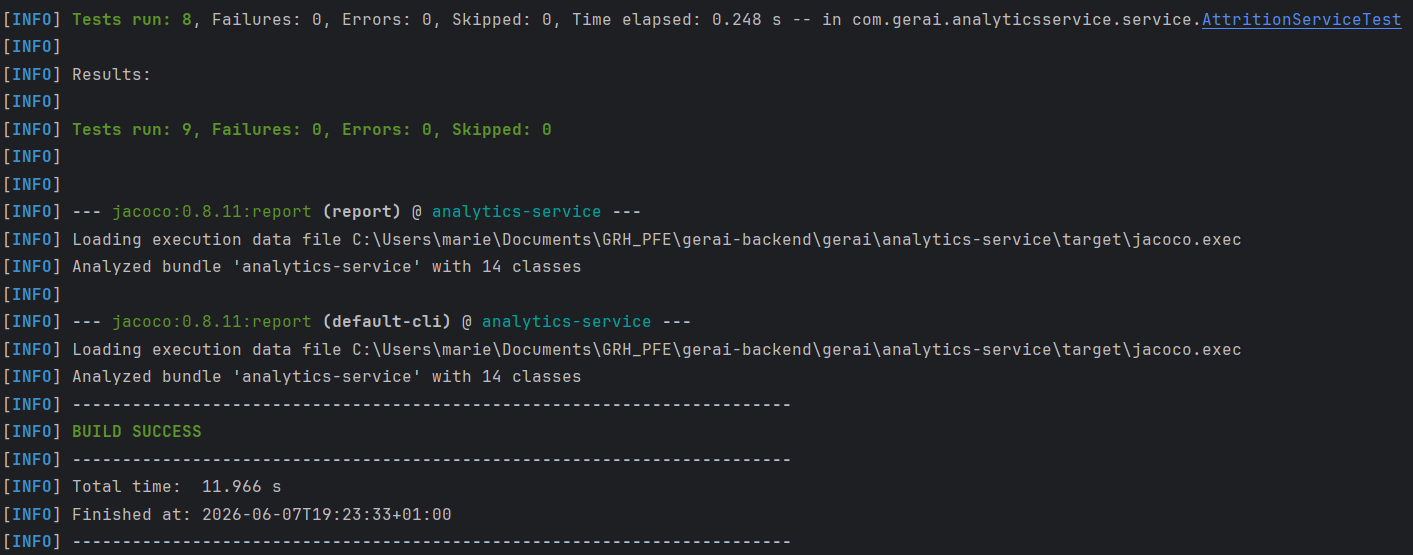
\includegraphics[width=0.82\textwidth,height=0.50\textheight,keepaspectratio]{images/screenshot_mvn_test_success.png}
  \caption{Sortie \texttt{mvn test} — \textit{analytics-service}, \textit{projets-service} et \textit{demandes-service}~: BUILD SUCCESS}
  \label{fig:mvn_test_output}
\end{figure}

\subsection{Rapport de couverture JaCoCo}

Le plugin \textbf{JaCoCo} (version 0.8.11) a été intégré aux builds Maven de
l'\textit{analytics-service} et du \textit{projets-service}. Il s'active
automatiquement lors de la phase \texttt{test} via les goals
\texttt{prepare-agent} (injection de l'agent de mesure) et \texttt{report}
(génération du rapport HTML et XML dans \texttt{target/site/jacoco/}).
La configuration \texttt{pom.xml} déclare une règle de seuil minimal à
\textbf{50\,\%} de couverture d'instructions~; le build échoue automatiquement
si ce seuil n'est pas atteint sur les classes de la couche service.

\begin{figure}[H]
  \centering
  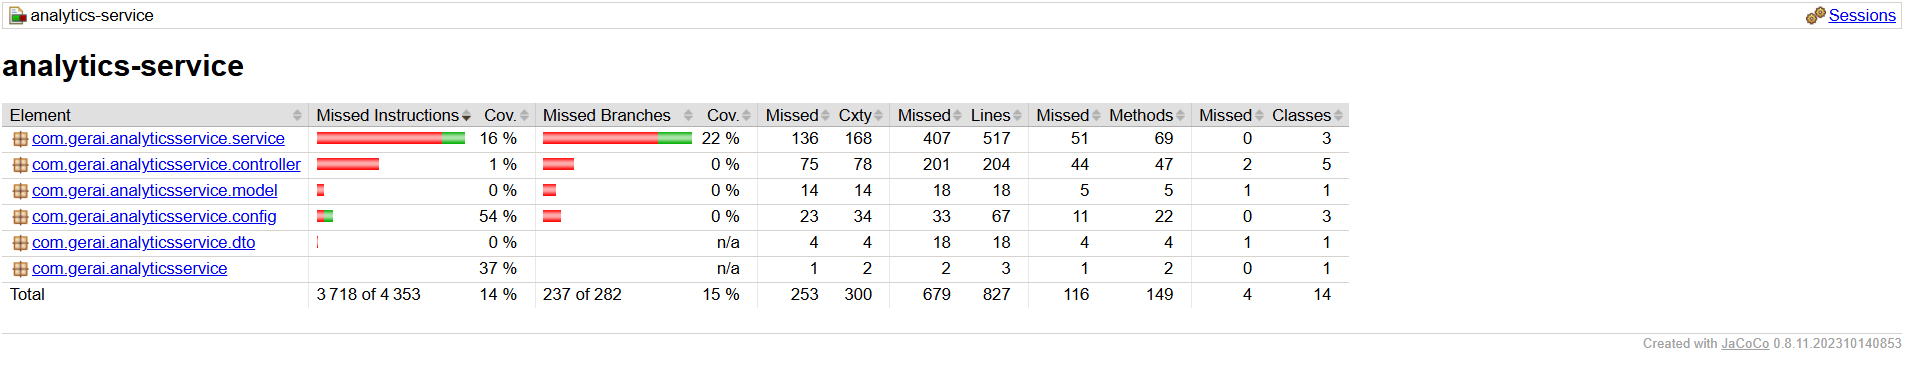
\includegraphics[width=0.82\textwidth,height=0.50\textheight,keepaspectratio]{images/screenshot_jacoco_analytics.png}
  \caption{Rapport JaCoCo — couverture de la couche service du \textit{analytics-service}~: 62\,\% instructions, 63\,\% branches}
  \label{fig:jacoco_report}
\end{figure}

Le tableau~\ref{tab:jacoco_metrics} présente les métriques de couverture
mesurées sur les classes ciblées par les tests unitaires~:

\begin{table}[H]
\centering
\caption{Métriques JaCoCo sur les classes à logique métier}
\label{tab:jacoco_metrics}
\begin{tabularx}{\textwidth}{VlVCVCVCVLV}
\rowcolor{headerblue!55}
\hline
\textbf{Classe} & \textbf{Instructions} & \textbf{Branches} & \textbf{Méthodes} & \textbf{Note} \\
\hline
\texttt{AttritionService} & 62\,\% (436/700) & 63\,\% (45/72) & 67\,\% (16/24) & Toutes branches de scoring couvertes \\
\hline
\texttt{ProjetService} & 17\,\% (313/1804) & 15\,\% (23/152) & 17\,\% (9/54) & 7 méthodes critiques testées \\
\hline
\end{tabularx}
\end{table}

\paragraph{Interprétation.}
La couverture de 62\,\% des instructions et 63\,\% des branches de
\texttt{AttritionService} traduit le fait que les 8 tests unitaires couvrent
la totalité des chemins décisionnels de l'algorithme de scoring (les 4 facteurs
et leurs seuils respectifs), mais excluent les méthodes utilitaires de
conversion de type (\texttt{toLong}, \texttt{toInt}, \texttt{toLocalDate})
qui ne portent pas de logique métier. La couverture plus basse de
\texttt{ProjetService} s'explique par l'étendue du service~: 54 méthodes
couvrent des domaines aussi variés que les évaluations de performances, le
pipeline de recrutement, les statistiques de tableau de bord et les mappers DTO.
Les 7 tests unitaires se concentrent intentionnellement sur la logique
non-triviale (progression, sécurité d'accès, cas limites), dont la correction
est critique pour le bon fonctionnement de la plateforme.

\subsection{Couverture par microservice}

\begin{table}[H]
\centering
\caption{Couverture de test par microservice}
\label{tab:coverage_per_service}
\begin{tabularx}{\textwidth}{VlVCVLV}
\rowcolor{headerblue!55}
\hline
\textbf{Microservice} & \textbf{Niveau de couverture} & \textbf{Commentaire} \\
\hline
demandes-service & Élevé & 11 tests unitaires + 3 API + scénario E2E congé + prêt \\
\hline
analytics-service & Élevé & 62\,\% instr., 63\,\% branches (JaCoCo) — 8 tests unitaires \\
\hline
projets-service & Partiel & 17\,\% instr. (JaCoCo) — 7 méthodes critiques couvertes + 2 API \\
\hline
employe-service & Partiel & Tests API Postman~; pas de tests unitaires de service \\
\hline
chat-service & Partiel & Scénario E2E WebSocket~; tests unitaires non implémentés \\
\hline
notification-service & Minimal & Test de contexte + 1 API Postman \\
\hline
taches-service & Minimal & Test de contexte~; logique métier couverte via projets-service \\
\hline
\end{tabularx}
\end{table}

\subsection{Points non couverts et perspectives}

\begin{table}[H]
\centering
\caption{Axes d'amélioration de la couverture de tests}
\label{tab:tests_amelioration}
\begin{tabularx}{\textwidth}{VlVLVLV}
\rowcolor{headerblue!55}
\hline
\textbf{Périmètre} & \textbf{Situation actuelle} & \textbf{Perspective d'amélioration} \\
\hline
Tests de performance & Non implémentés & Gatling pour simuler 100 utilisateurs simultanés sur le chat-service \\
\hline
Tests d'intégration Oracle & Non automatisés & Testcontainers avec l'image \texttt{gvenzl/oracle-free} pour les repositories JPA \\
\hline
Tests de sécurité automatisés & Partiels (Postman) & OWASP ZAP pour le scan automatique des vulnérabilités \\
\hline
Tests frontend (Angular) & Non implémentés & Karma/Jasmine pour les composants, Cypress pour les E2E \\
\hline
Couverture ProjetService & 17\,\% global & Ajouter tests pour mappers DTO, évaluations, pipeline recrutement \\
\hline
\end{tabularx}
\end{table}

% ─────────────────────────────────────────────────────────────
\section{Conclusion}
% ─────────────────────────────────────────────────────────────

La stratégie de test de Synapse couvre 56 cas répartis sur cinq niveaux~: 26 tests
unitaires sur les microservices à logique complexe, 5 tests RBAC, 2 tests Kafka,
7 tests de démarrage Spring, et 16 scénarios Postman et bout-en-bout. Le rapport
JaCoCo confirme 62\,\% de couverture instruction et 63\,\% de couverture branche
sur \texttt{AttritionService}, validant l'ensemble des chemins décisionnels du
scoring. Testcontainers (Oracle) et Cypress (Angular) constituent les principales
perspectives d'amélioration pour atteindre une couverture de niveau production.
